
%%%%%%%%%%%%%%%%%%%%%%%%%%%%%
% Standard header for working papers
%
% WPHeader.tex
%
%%%%%%%%%%%%%%%%%%%%%%%%%%%%%

\documentclass[11pt]{article}



%%%%%%%%%%%%%%%%%%%%%%%%%%
%% TEMPLATES
%%%%%%%%%%%%%%%%%%%%%%%%%%


% Simple Tabular

%\begin{tabular}{ |c|c|c| } 
% \hline
% cell1 & cell2 & cell3 \\ 
% cell4 & cell5 & cell6 \\ 
% cell7 & cell8 & cell9 \\ 
% \hline
%\end{tabular}





%%%%%%%%%%%%%%%%%%%%%%%%%%
%% Packages
%%%%%%%%%%%%%%%%%%%%%%%%%%



% encoding 
\usepackage[utf8]{inputenc}
\usepackage[T1]{fontenc}


% general packages without options
\usepackage{amsmath,amssymb,amsthm,bbm}

% graphics
\usepackage{graphicx,transparent,eso-pic}

% text formatting
\usepackage[document]{ragged2e}
\usepackage{pagecolor,color}
%\usepackage{ulem}
\usepackage{soul}


% conditions
\usepackage{ifthen}


\usepackage{booktabs}
\usepackage{threeparttable}



%%%%%%%%%%%%%%%%%%%%%%%%%%
%% Maths environment
%%%%%%%%%%%%%%%%%%%%%%%%%%

%\newtheorem{theorem}{Theorem}[section]
%\newtheorem{lemma}[theorem]{Lemma}
%\newtheorem{proposition}[theorem]{Proposition}
%\newtheorem{corollary}[theorem]{Corollary}

%\newenvironment{proof}[1][Proof]{\begin{trivlist}
%\item[\hskip \labelsep {\bfseries #1}]}{\end{trivlist}}
%\newenvironment{definition}[1][Definition]{\begin{trivlist}
%\item[\hskip \labelsep {\bfseries #1}]}{\end{trivlist}}
%\newenvironment{example}[1][Example]{\begin{trivlist}
%\item[\hskip \labelsep {\bfseries #1}]}{\end{trivlist}}
%\newenvironment{remark}[1][Remark]{\begin{trivlist}
%\item[\hskip \labelsep {\bfseries #1}]}{\end{trivlist}}

%\newcommand{\qed}{\nobreak \ifvmode \relax \else
%      \ifdim\lastskip<1.5em \hskip-\lastskip
%      \hskip1.5em plus0em minus0.5em \fi \nobreak
%      \vrule height0.75em width0.5em depth0.25em\fi}


%% Commands

\newcommand{\noun}[1]{\textsc{#1}}


%% Math

% Operators
\DeclareMathOperator{\Cov}{Cov}
\DeclareMathOperator{\Var}{Var}
\DeclareMathOperator{\E}{\mathbb{E}}
\DeclareMathOperator{\Proba}{\mathbb{P}}

\newcommand{\Covb}[2]{\ensuremath{\Cov\!\left[#1,#2\right]}}
\newcommand{\Eb}[1]{\ensuremath{\E\!\left[#1\right]}}
\newcommand{\Pb}[1]{\ensuremath{\Proba\!\left[#1\right]}}
\newcommand{\Varb}[1]{\ensuremath{\Var\!\left[#1\right]}}

% norm
\newcommand{\norm}[1]{\left\lVert #1 \right\rVert}



% argmin
\DeclareMathOperator*{\argmin}{\arg\!\min}


% amsthm environments
\newtheorem{definition}{Definition}
\newtheorem{proposition}{Proposition}
\newtheorem{assumption}{Assumption}

%% graphics

% renew graphics command for relative path providment only ?
%\renewcommand{\includegraphics[]{}}








% geometry
\usepackage[margin=2cm]{geometry}

% layout : use fancyhdr package
\usepackage{fancyhdr}
\pagestyle{fancy}

\makeatletter

\renewcommand{\headrulewidth}{0.4pt}
\renewcommand{\footrulewidth}{0.4pt}
\fancyhead[RO,RE]{\textit{Working Paper}}
\fancyhead[LO,LE]{CASA/ISC-PIF}
\fancyfoot[RO,RE] {\thepage}
\fancyfoot[LO,LE] {\noun{J. Raimbault}}
\fancyfoot[CO,CE] {}

\makeatother


%%%%%%%%%%%%%%%%%%%%%
%% Begin doc
%%%%%%%%%%%%%%%%%%%%%

\begin{document}






\begin{document}

%%% Start of article front matter
\begin{frontmatter}

\begin{fmbox}
\dochead{Research}

\title{Citation network analysis of urban modeling research}

\author[
   addressref={aff1,aff2,aff3},                   % id's of addresses, e.g. {aff1,aff2}
   corref={aff1},                       % id of corresponding address, if any
   %noteref={n1},                        % id's of article notes, if any
   email={juste.raimbault@polytechnique.edu}   % email address
]{\inits{JR}\fnm{Juste} \snm{Raimbault}}
\author[
   addressref={aff2},
   email={m.vanhoof@ucl.ac.uk}
]{\inits{MV}\fnm{Maarten} \snm{Vanhoof}}
\author[
   addressref={aff2},
   email={m.batty@ucl.ac.uk}
]{\inits{MB}\fnm{Michael} \snm{Batty}}


\address[id=aff1]{%                           % unique id
  \orgname{UPS CNRS 3611 ISC-PIF}, % university, etc
  %\street{113 rue Nationale},                     %
  %\postcode{75013}                                % post or zip code
  \city{Paris},                              % city
  \cny{France}                                    % country
}
\address[id=aff2]{%
  \orgname{CASA, UCL},
  %\street{},
  %\postcode{}
  \city{London},
  \cny{UK}
}
\address[id=aff3]{%
  \orgname{UMR CNRS 8504 G{\'e}ographie-cit{\'e}s},
  %\street{},
  %\postcode{}
  \city{Paris},
  \cny{France}
}

\begin{artnotes}
%\note{Sample of title note}     % note to the article
%\note[id=n1]{Equal contributor} % note, connected to author
\end{artnotes}

\end{fmbox}% comment this for two column layout

\begin{abstractbox}

\begin{abstract} % abstract
%\parttitle{First part title} %if any
Several modeling approaches to the evolution of urban and territorial environments have been introduced in the literature, providing complementary viewpoints and methods. This paper contributes to the mapping of this scientific landscape by a citation network analysis. Taking the case study of two landmark types of operational models, namely microsimulation models and land-use transport interaction model, we construct an initial corpus through keyword requests. The backward citation network is then reconstructed up to depth two, yielding a network with $4.54\cdot 10^5$ nodes and $8.07\cdot 10^5$ citation links. Community detection in the network provides endogenous disciplines and approaches, including a broader scope than the initial corpus, with for example spatial statistics and agent-based modeling. We construct measures of interdisciplinarity to identify bridge papers, and investigate possible missing connections. We illustrate these more particularly with the interface of microsimulation, agent-based modeling and land-use transport models, and discuss potential coupling of models filling this gap. We show therein how potential research directions can be unveiled through citation network analysis and provide partial maps of science in the field of urban modeling, which can be used by researchers and practitioners to better contextualize their modeling approaches.
\end{abstract}

\begin{keyword}
\kwd{citation network}
\kwd{interdisciplinarity}
\kwd{urban modeling}
\kwd{land-use transport interaction models}
\kwd{microsimulation models}
\end{keyword}


\end{abstractbox}
%
%\end{fmbox}% uncomment this for twcolumn layout

\end{frontmatter}


%%%%%%%%%%%%%%%%%%%%%%
\section*{Introduction}

Urban modeling, defined broadly as quantitative modeling and simulation aiming at understanding urban processes, has always been a highly multidisciplinary and interdisciplinary subject \cite{ramadier2004transdisciplinarity}. Indeed, several disciplines ranging from Urban Economics~\cite{krugman1998s} to Quantitative Urban Geography~\cite{pumain2017geography} or Urban Planning~\cite{knowles2016sir} provide complementary viewpoints by studying different dimensions of urban phenomena. Despite sometimes converging issues, bridges remain rather rare, such as integrating approaches such as the Science of Cities introduced by \cite{batty2013new}. One crucial question in that context is to what extent these different approaches to modeling urban issues may be complementary, and what may the potentially fertile couplings in terms of producing new knowledge. Indeed, a good knowledge of the scientific landscape, or in other terms a certain level of reflexivity, is crucial for urban modeling studies since as \cite{batty2019map} points out, models become digital twins of modelled systems which themselves play a role in the studied system.


While problem-specific entries, i.e. studying a specific system and correspondences between some of its models, will shed light on thematic aspects of this question, one can also consider the knowledge landscape in itself to identify existing approaches and potential links. This paper investigates urban modeling at this second level, and proposes to build a mapping of some approaches in urban modeling through citation network analysis. Quantitative studies of science have a long history such as in sociology of science~\cite{barnes1982science}, but recent works have witnessed significant progress driven by the emergence of large dataset and digital libraries. Maps of science have been constructed \cite{boyack2005mapping} and a ``Science of Science'' would be appearing as an interdisciplinary field~\cite{fortunato2018science}. We situate here within that stream of research, using network analysis to better understand the structure of knowledge around the topic of urban modeling.


Citation network has to the best of our knowledge never been systematically applied to the subject of urban modeling, in the sense of a broad and general coverage and large dataset. Specific urban issues were however studied through citation network analysis. \cite{van2016pacifying} map the debate around urban region polycentricity. \cite{raimbault2019exploration} develops a multilayer analysis, coupling citations with semantic content, of the neighborhood of a geography journal, including clusters tackling urban questions.

%\cite{giatsidis2019rooted} propose  new measures based on subgraph density for citation networks

We construct a large corpus of papers, linked through backward citations.
Our contribution relies on the following points: (i) the open dataset we make available can be of significant interest for researcher interested in urban modeling; (ii) we map a broad part of approaches to urban modeling, and more particularly clarify the relations between microsimulation, land-use transport modeling, and agent-nased modeling.
% (i) sensitivity analysis - info to reconstruct discipline with such empirical data ?
% (ii) some methodological insights depending on what we do ?
% (iii) results on urban modeling in themselves <- Maybe insist only on that ?


The rest of the paper is organized as follows. We first describe the construction of the dataset, i.e. the initial assumptions and data collection process, and the filtering steps to work on a relevant network. We then study its sensitivity to construction parameters, what allows to comment on endogenous disciplines and study the evolution of communities in time. We finally discuss the implication of these results, for example in the context of coupling approaches.


%%%%%%%%%%%%%%%%%%%%%%
\section*{Dataset construction}

\subsection*{Initial seed}

We propose a multiple keyword entry to build a broad corpus, on complementary but distinct approaches. This will ensure first that the collected data is representative due to the corpus size limitations, but secondly that potential couplings are included. % REFORMULATE

The initial keyword requests we use are the following: ``microsimulation'', ``microsimulation model'', ``spatial microsimulation model'', ``urban microsimulation model'', ``transport microsimulation model'', ``land use transport interaction model''.


Our corpus is surely not exhaustive to urban modeling as we focused on the aforementioned two main entries, and other requests such as ``urban geosimulation'', ``urban growth model'', ``urban agent based model'' would also be relevant. We expect for example, following \cite{wise2016transportation}, to have a strong overlap with our corpus and a potential corpus related to agent-based modeling. Similarly, other sub-fields of urban modeling such as cellular automata \cite{white1993cellular} or geosimulation \cite{benenson2004geosimulation} are expected to be highly interwined with our corpus from a thematic viewpoint.
%urban agent based model, spatial interaction model, spatial interaction agent based model, geosimulation, urban geosimulation, urban cellular automata, urban growth model, urban land use change model, urban land use model


\subsection*{Citation network collection}


%%%%%
% full network
%IGRAPH 9ceae4d DN-- 467608 834253 -- 
%+ attr: name (v/c), title (v/c), year (v/c), depth (v/n), priority (v/n), horizontalDepth (v/c), citingFilled (v/c), lang (v/c)



\subsection*{Network filtering}

Language statistics (detected using titles). We do not include in our analysis any semantic analysis and thus do not filter on language of papers. Note that as we work on citation networks, cross-language citations are a common feature and different languages will not produce isolated clusters. In any case, a language detection with the python package \texttt{polyglot} confirms that most of the corpus is in English (86.6\%), secondary main language being Mandarin (4.7\%), Spanish (1.8\%), German (1.6\%), French (1.2\%) and Portuguese (1.2\%).
% possible additional analysis by isolating language subnetworks - checking modularity of language communities ?. Typically: Chinese article are only cited by other Chinese articles. similar but less strong effect with French

%     Czech    Swedish   Galician      Dutch Indonesian    Turkish   
% 0.1129035  0.1259161  0.1274470  0.1672503  0.1693553  0.2309738  
% Italian    Russian     Korean     Polish 
%0.3155558  0.3832979  0.3987982  0.4384102 
%  Japanese Portuguese     French     German    Spanish  
% 0.4720899  1.2195495  1.2339017  1.6231318  1.7783263 
% Chinese    English 
%4.6506688 86.5524236



% components(citation)$csize
% 466610    517      5    246     53     57      6     58      3     10      7      5      7     15      3      2     2      2
%  2nd comp 517 -> breast cancer ! (should come from "microsimulation" req alone
% 4th component : agriculture / soils

We keep the giant connected cluster of the resulting network, which covers 99.8\% of all nodes (yielding at this step $\left|V\right| = 466,610$ nodes). Inspection of removed clusters confirms that these are not relevant to urban issues (medical or chemistry microsimulations for example). Because of the way citation networks are organized and how our dataset was constructed, the full network contains a large part of ``graps'' which consist in several uncited papers citing the same one. We choose thus to work on the ``core'' of the network, which we construct by successively removing nodes of degree less or equal to one until there are no more such nodes.


%%%%%%%%%%%%%%%%%%%%%%
\section*{Mapping the scientific landscape}

\subsection*{Sensitivity analysis}

% check modularity = f(horizontal and vertical depth) : insight into the relevant number of initially requested papers ; Sensitivity of 'width' of paper. Width=the amount of hits in google scholar we use ; Sensitivity of the used key words => all in same analysis

Before being able to proceed to any thematically relevant network analysis, a sensitivity analysis of network properties as a function of construction parameters is necessary. More particularly, the results may be strongly dependent on the number of search results retained and on the requests used. This preliminary aims at checking this dependency and extract the most robust subnetwork possible for the rest of the analysis.

We first investigate how network topology varies as a function of horizontal depth.


%%%%%%%%
\begin{figure}
    \centering
    \includegraphics{}
    \caption{}
    \label{fig:modularity-hdepth}
\end{figure}
%%%%%%%%


We then assess that a certain level of overlap exists between the sub-networks originating from different initial requests. As shown in Fig.~\ref{fig:coverage-hdepth}

%%%%%%%%
\begin{figure}
    \centering
    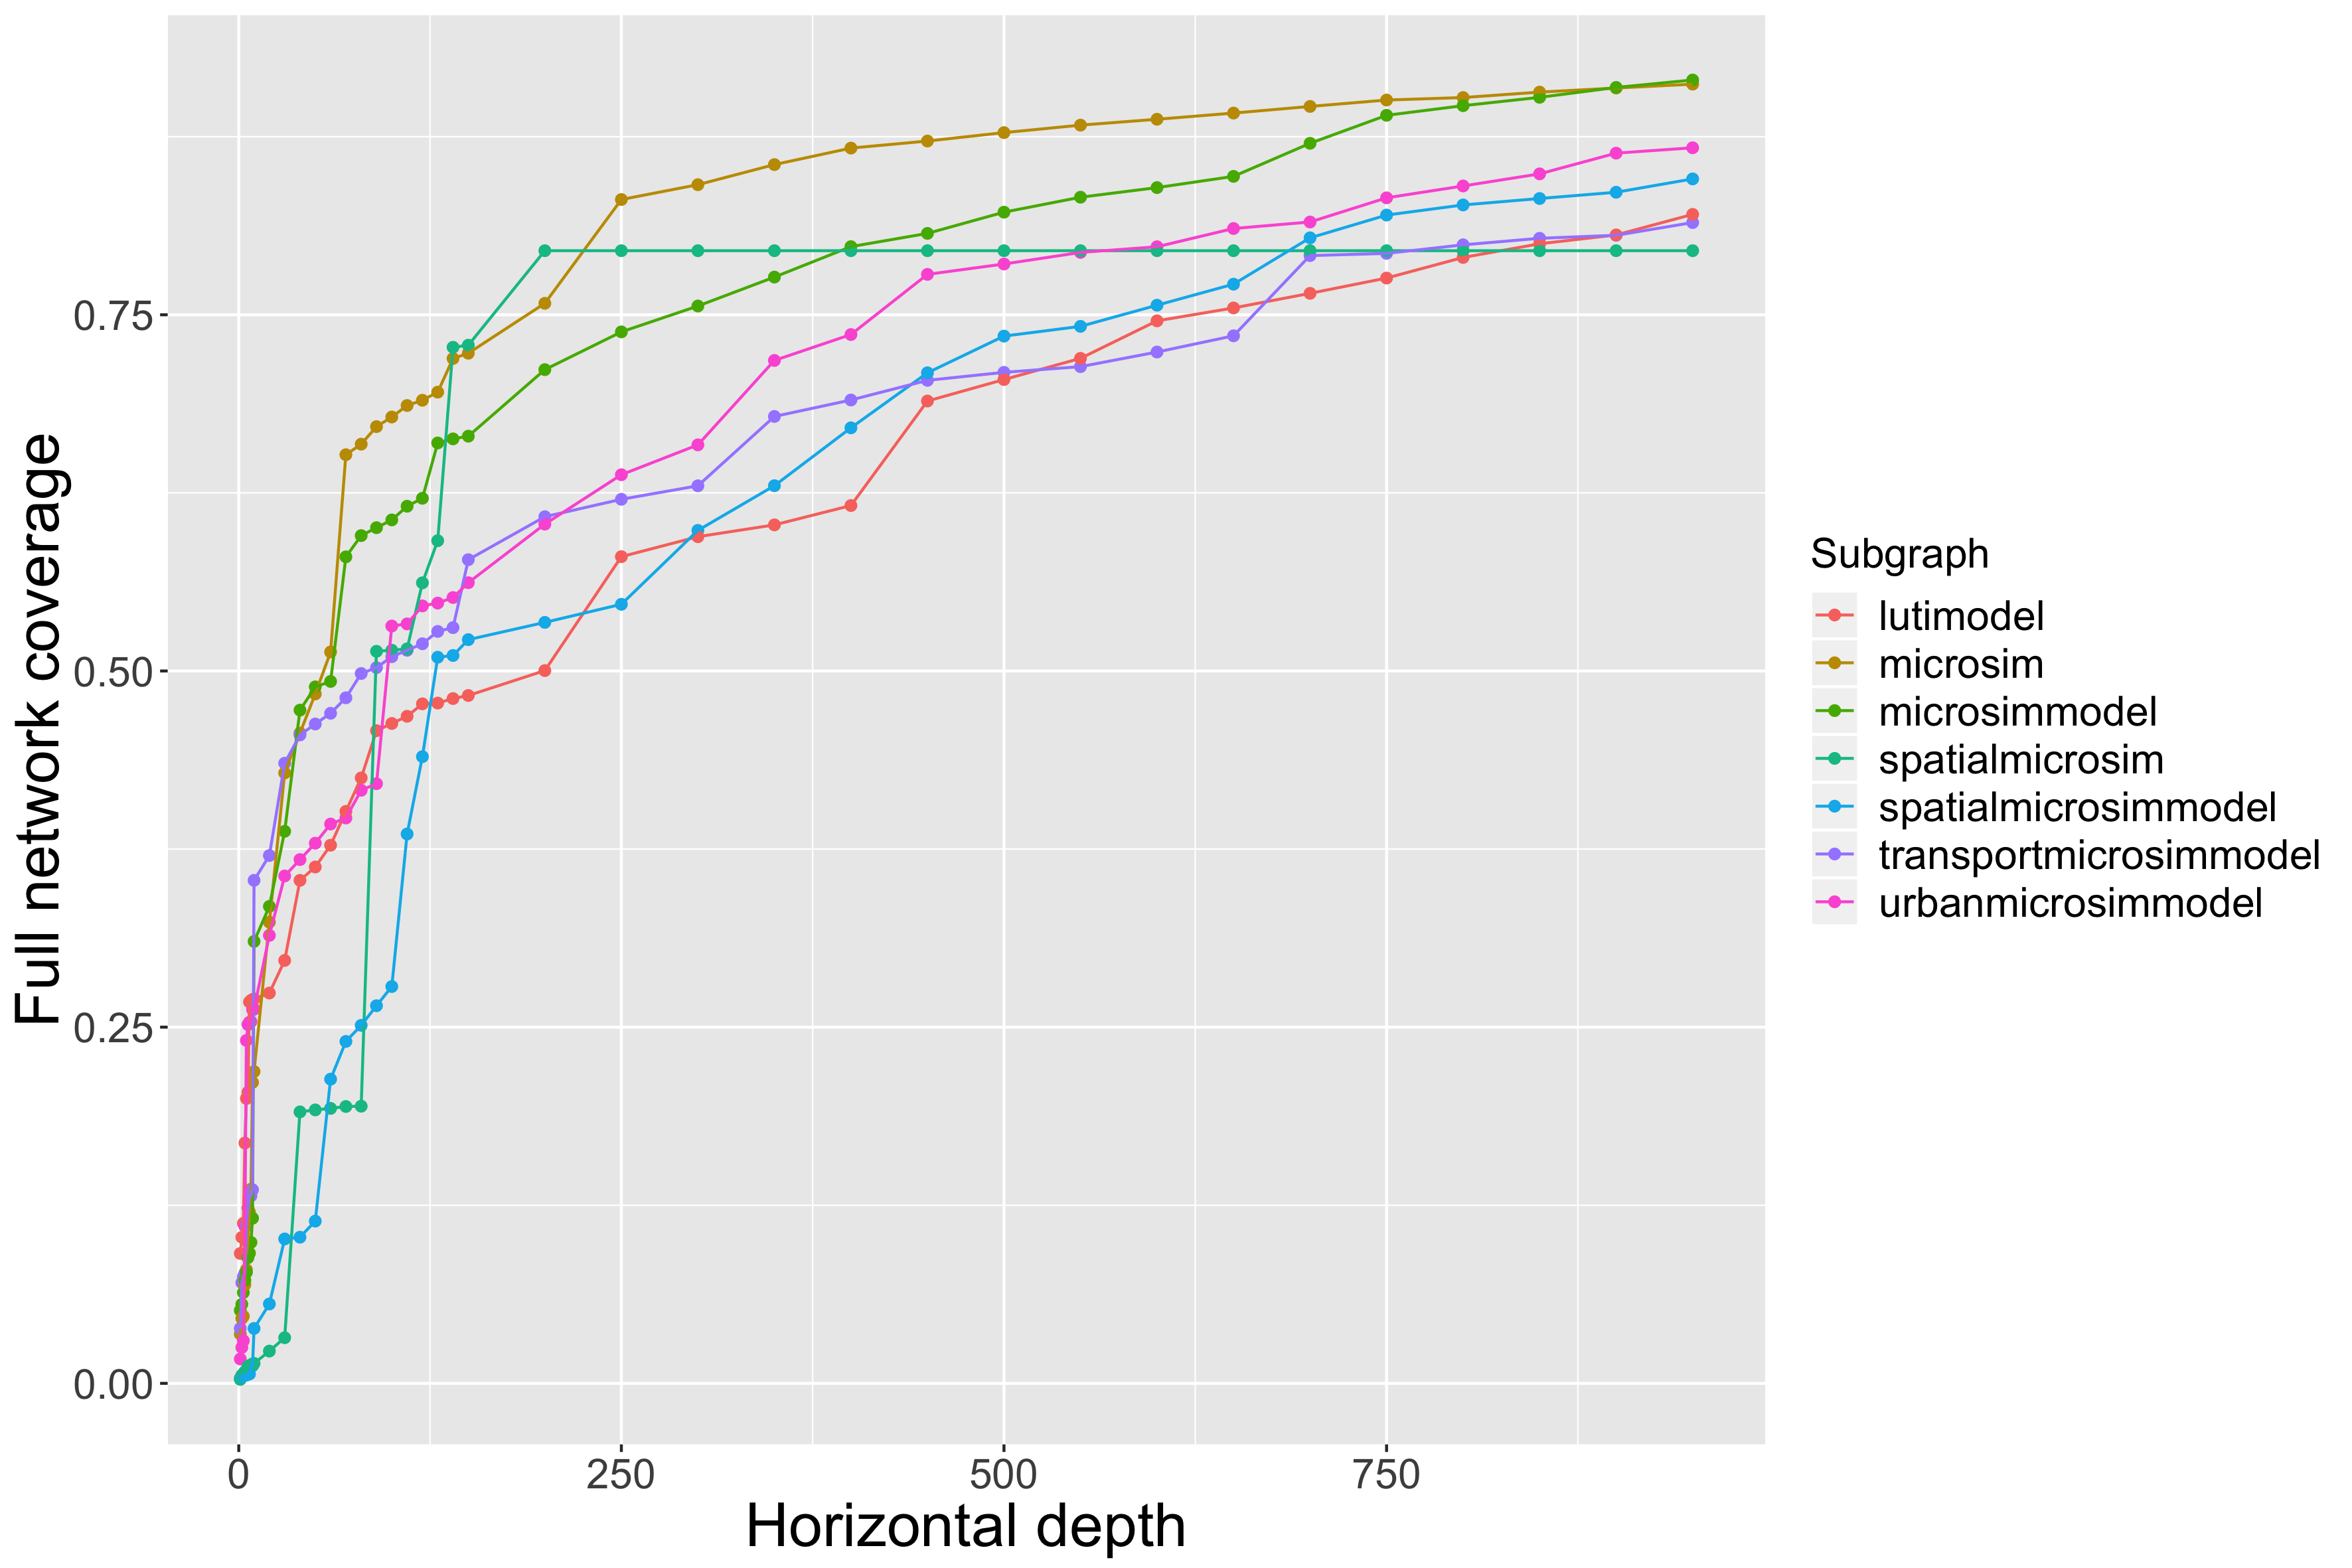
\includegraphics{figures/coveragesubnws.png}
    \caption{}
    \label{fig:coverage-hdepth}
\end{figure}
%%%%%%%%


\subsection*{Reconstructing endogenous disciplines}

% cluster sizes
The distribution of community size is fat-tailed in a power-law manner


% Investigate the occurrence of some terms and their membership towards different clusters


%Measuring interdisciplinarity

%The existence of clusters related to different tools or techniques (e.g. Matsim)



\subsection*{Temporal analysis of communities}
% Investigate the temporality of the nodes and links % TODO Maarten

% Percolation of links based on frequency of citations or maybe on time also -> is percolation useful at this point ?
 


%\subsection*{A case study: LUTI and microsimulation}




%%%%%%%%%%%%%%%%%%%%%%
\section*{Discussion}

% possible developments:
% with semantic content : 
%Text mining of abstracts to automatically denote -content- of the clusters\
% Investigate the location of certain authors\\
% Investigate the propagation of some of the most important works\\
% Investigate the content of 'connecting' papers

%Can we reconstruct the cluster based on iterative search terms in google scholar? -- see where the convergence point is for certain terms


% TODO : possible subject for Tongji workshop (search chinese kws)



%%%%%%%%%%%%%%%%%%%%%%
\section*{Conclusion}




%%%%%%%%%%%%%%%%%%%%%%%%%%%%%%%%%%%%%%%%%%%%%%
%%                                          %%
%% Backmatter begins here                   %%
%%                                          %%
%%%%%%%%%%%%%%%%%%%%%%%%%%%%%%%%%%%%%%%%%%%%%%

\begin{backmatter}

%\section*{Competing interests}
%  The authors declare that they have no competing interests.

%\section*{Author's contributions}
%    Text for this section \ldots

%\section*{Acknowledgements}
%  Text for this section \ldots
%%%%%%%%%%%%%%%%%%%%%%%%%%%%%%%%%%%%%%%%%%%%%%%%%%%%%%%%%%%%%
%%                  The Bibliography                       %%
%%                                                         %%
%%  Bmc_mathpys.bst  will be used to                       %%
%%  create a .BBL file for submission.                     %%
%%  After submission of the .TEX file,                     %%
%%  you will be prompted to submit your .BBL file.         %%
%%                                                         %%
%%                                                         %%
%%  Note that the displayed Bibliography will not          %%
%%  necessarily be rendered by Latex exactly as specified  %%
%%  in the online Instructions for Authors.                %%
%%                                                         %%
%%%%%%%%%%%%%%%%%%%%%%%%%%%%%%%%%%%%%%%%%%%%%%%%%%%%%%%%%%%%%

% if your bibliography is in bibtex format, use those commands:
\bibliographystyle{bmc-mathphys} % Style BST file (bmc-mathphys, vancouver, spbasic).
\bibliography{biblio}      % Bibliography file (usually '*.bib' )
% for author-year bibliography (bmc-mathphys or spbasic)
% a) write to bib file (bmc-mathphys only)
% @settings{label, options="nameyear"}
% b) uncomment next line
%\nocite{label}

% or include bibliography directly:
% \begin{thebibliography}
% \bibitem{b1}
% \end{thebibliography}




%%%%%%%%%%%%%%%%%%%%%%%%%%%%%%%%%%%
%%                               %%
%% Figures                       %%
%%                               %%
%% NB: this is for captions and  %%
%% Titles. All graphics must be  %%
%% submitted separately and NOT  %%
%% included in the Tex document  %%
%%                               %%
%%%%%%%%%%%%%%%%%%%%%%%%%%%%%%%%%%%

%%
%% Do not use \listoffigures as most will included as separate files

%  \begin{figure}[h!]
%  \caption{\csentence{Sample figure title.}
%      A short description of the figure content
%      should go here.}
%      \end{figure}

%\begin{figure}[h!]
%  \caption{\csentence{Sample figure title.}
%      Figure legend text.}
%      \end{figure}

%%%%%%%%%%%%%%%%%%%%%%%%%%%%%%%%%%%
%%                               %%
%% Tables                        %%
%%                               %%
%%%%%%%%%%%%%%%%%%%%%%%%%%%%%%%%%%%

%\begin{table}[h!]
%\caption{Sample table title. This is where the description of the table should go.}
%      \begin{tabular}{cccc}
%        \hline
%           & B1  &B2   & B3\\ \hline
%        A1 & 0.1 & 0.2 & 0.3\\
%        A2 & ... & ..  & .\\
%        A3 & ..  & .   & .\\ \hline
%      \end{tabular}
%\end{table}

%%%%%%%%%%%%%%%%%%%%%%%%%%%%%%%%%%%
%%                               %%
%% Additional Files              %%
%%                               %%
%%%%%%%%%%%%%%%%%%%%%%%%%%%%%%%%%%%

%\section*{Additional Files}
%  \subsection*{Additional file 1 --- Sample additional file title}
%    Additional file descriptions text (including details of how to   view the file, if it is in a non-standard format or the file extension).  This might   refer to a multi-page table or a figure.
% \subsection*{Additional file 2 --- Sample additional file title}
%    Additional file descriptions text.


\end{backmatter}
\end{document}



